% !TEX spellcheck = en_US



% ~~~~~~~~~~~~~~~~~~~~~~~~~~~~~~~~~~~~~~~ V
% (NC) 2026 Haluk Bingol
% github.com/halukbingol/LaTeX-Templates
%
% Licensees may copy, distribute, display, and perform the work and make derivative works 
% and remixes based on it only for non-commercial purposes. 
% ~~~~~~~~~~~~~~~~~~~~~~~~~~~~~~~~~~~~~~~ A




% =====================================================================
%  Linked Lists -- The Presentation
%  ---------------------------------------------------------------------
%  Built on hblib/Template/hblibTemplate.tex with the libraries in ../../hblib/.
%  Programs and their real outputs are in codeoutput/.
% =====================================================================

\documentclass[aspectratio=169,10pt,compress]{beamer}

% ~~~~~~~~~~~~~~~~~~~~~~~~~~~~~~~~~~~~~~~~~~~~~~~~~~~~~~~~~~~~~~~~~ V hblib
	\usepackage{../../hblib/hblibPresentation}
	\usepackage{../../hblib/hblibCodeoutput}
	\usepackage{../../hblib/hblibDatastructures}
% ~~~~~~~~~~~~~~~~~~~~~~~~~~~~~~~~~~~~~~~~~~~~~~~~~~~~~~~~~~~~~~~~~ A hblib


\usepackage[T1]{fontenc}
\usepackage{lmodern}
\usepackage{booktabs}

% long Java lines: wrap instead of running off the frame
\lstset{columns=fixed, breaklines=true, breakatwhitespace=false}

\title{Linked Lists}
\subtitle{The Presentation}
\author[Alpaydin]{Ruhan Alpaydin}
\institute[FCIS]{Faculty of Computer and Information Sciences\\Yeditepe University}
\date{{\tiny \hbTimeStamp}}

\begin{document}




% ~~~~~~~~~~~~~~~~~~~~~~~~~~~~~~~~~~~~~~ V frm
\begin{frame}[t,fragile]
  \titlepage
\end{frame}
% ~~~~~~~~~~~~~~~~~~~~~~~~~~~~~~~~~~~~~~ A frm




% ~~~~~~~~~~~~~~~~~~~~~~~~~~~~~~~~~~~~~~ V frm
\begin{frame}[t,fragile] \frametitle{Outline}
  \begin{columns}[T]
    \begin{column}{0.48\textwidth}
      \tableofcontents[sections={1-5}, hideallsubsections]
    \end{column}
    \begin{column}{0.48\textwidth}
      \tableofcontents[sections={6-9}, hideallsubsections]
    \end{column}
  \end{columns}
\end{frame}
% ~~~~~~~~~~~~~~~~~~~~~~~~~~~~~~~~~~~~~~ A frm

% ~~~~~~~~~~~~~~~~~~~~~~~~~~~~~~~~~~~~~~ V
\hSection[Idea]{Why a linked list?}
% ~~~~~~~~~~~~~~~~~~~~~~~~~~~~~~~~~~~~~~ A




% ~~~~~~~~~~~~~~~~~~~~~~~~~~~~~~~~~~~~~~ V frm
\begin{frame}[t,fragile] \frametitle{Two ways to store a sequence}
  \begin{columns}[T]
    \begin{column}{0.5\textwidth}
      \begin{block}{Array}
        \small
        \hCode{a[0]}, \hCode{a[1]}, \dots, \hCode{a[n-1]} in one block.\\
        Jump to \hCode{a[k]} in $O(1)$.\\
        Insert or delete in the middle: move $n-k$ elements.
      \end{block}
    \end{column}
    \begin{column}{0.46\textwidth}
      \begin{block}{Linked list}
        \small
        Each element lives in its own \textbf{node}, with a
        \hCode{next} reference.\\
        Jump to position $k$: walk from the head ($O(k)$).\\
        Insert or delete: change two references.
      \end{block}
    \end{column}
  \end{columns}
  \vspace{0.4em}
  \small
  \hRemark{Neither is better}: an array is better when you know the
  position; a linked list is better when you know the node.
\end{frame}
% ~~~~~~~~~~~~~~~~~~~~~~~~~~~~~~~~~~~~~~ A frm




% ~~~~~~~~~~~~~~~~~~~~~~~~~~~~~~~~~~~~~~ V frm
\begin{frame}[t,fragile] \frametitle{What a node is}
  \begin{center}\small
  \begin{tabular}{@{}lll@{}}
    \toprule
    \textbf{Field} & \textbf{Meaning} & \textbf{Java} \\
    \midrule
    data  & the value being stored     & \hCode{int iData} \\
    next  & a reference to the next node, or \hCode{null} & \hCode{Link next} \\
    \bottomrule
  \end{tabular}
  \end{center}
  \vspace{0.4em}
  \small
  A linked list is a chain of such nodes (links). The list holds a single
  reference, \hCode{first}, to the head of the chain. The last node
  in the chain has \hCode{next == null}.
  \vspace{0.6em}

  \begin{center}
  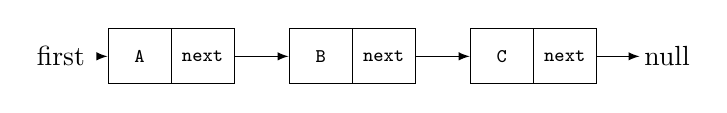
\begin{tikzpicture}
    \node at (-1.4,0) {\hCode{first}};
    \node[draw, minimum width=1.6cm, minimum height=0.7cm] (a) at (0,0) {};
    \node[font=\ttfamily\scriptsize] at (-0.4,0) {A};
    \node[font=\ttfamily\scriptsize] at ( 0.4,0) {next};
    \draw (a.north) -- (a.south);
    \node[draw, minimum width=1.6cm, minimum height=0.7cm] (b) at (2.3,0) {};
    \node[font=\ttfamily\scriptsize] at (1.9,0) {B};
    \node[font=\ttfamily\scriptsize] at (2.7,0) {next};
    \draw (b.north) -- (b.south);
    \node[draw, minimum width=1.6cm, minimum height=0.7cm] (c) at (4.6,0) {};
    \node[font=\ttfamily\scriptsize] at (4.2,0) {C};
    \node[font=\ttfamily\scriptsize] at (5.0,0) {next};
    \draw (c.north) -- (c.south);
    \node at (6.3,0) {\hCode{null}};
    \draw[-latex] (-0.85,0) -- (a.west);
    \draw[-latex] (a.east)  -- (b.west);
    \draw[-latex] (b.east)  -- (c.west);
    \draw[-latex] (c.east)  -- (5.95,0);
  \end{tikzpicture}
  \end{center}
  \vspace{0.2em}
  \small This list has three nodes: A, B, C, then \hCode{null}.
\end{frame}
% ~~~~~~~~~~~~~~~~~~~~~~~~~~~~~~~~~~~~~~ A frm


% ~~~~~~~~~~~~~~~~~~~~~~~~~~~~~~~~~~~~~~ V frm
\begin{frame}[t,fragile] \frametitle{Structure of a singly linked list}
  \begin{center}
  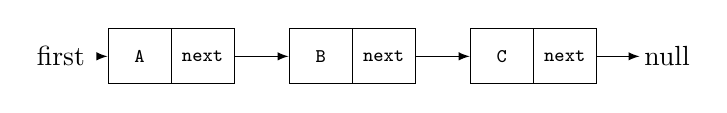
\begin{tikzpicture}
    \node at (-1.4,0) {\hCode{first}};
    \node[draw, minimum width=1.6cm, minimum height=0.7cm] (a) at (0,0) {};
    \node[font=\ttfamily\scriptsize] at (-0.4,0) {A};
    \node[font=\ttfamily\scriptsize] at ( 0.4,0) {next};
    \draw (a.north) -- (a.south);
    \node[draw, minimum width=1.6cm, minimum height=0.7cm] (b) at (2.3,0) {};
    \node[font=\ttfamily\scriptsize] at (1.9,0) {B};
    \node[font=\ttfamily\scriptsize] at (2.7,0) {next};
    \draw (b.north) -- (b.south);
    \node[draw, minimum width=1.6cm, minimum height=0.7cm] (c) at (4.6,0) {};
    \node[font=\ttfamily\scriptsize] at (4.2,0) {C};
    \node[font=\ttfamily\scriptsize] at (5.0,0) {next};
    \draw (c.north) -- (c.south);
    \node at (6.3,0) {\hCode{null}};
    \draw[-latex] (-0.85,0) -- (a.west);
    \draw[-latex] (a.east)  -- (b.west);
    \draw[-latex] (b.east)  -- (c.west);
    \draw[-latex] (c.east)  -- (5.95,0);
  \end{tikzpicture}
  \end{center}
  \vspace{0.4em}
  \begin{itemize}\small
    \item One reference (\hCode{first}) is enough to find every node.
    \item The list has no \hCode{last} unless you add one.
    \item Every node is reached through the previous node's \hCode{next}.
  \end{itemize}
\end{frame}
% ~~~~~~~~~~~~~~~~~~~~~~~~~~~~~~~~~~~~~~ A frm




% ~~~~~~~~~~~~~~~~~~~~~~~~~~~~~~~~~~~~~~ V frm
\begin{frame}[t,fragile] \frametitle{You can only walk forward}
  \begin{block}{Sequential access}
    \small
    To reach position $k$, start at \hCode{first} and follow
    \hCode{next} $k$ times. \hRemark{There is no \texttt{a[k]} in a linked list.}
  \end{block}
  \vspace{0.3em}
  \begin{itemize}\small
    \item Iteration is the normal way to visit every element.
    \item Any algorithm that jumps by index is the wrong fit.
    \item The JDK's \hCode{LinkedList.get(i)} is $O(i)$, which is why
          you use it as a \hCode{Deque}, not as a \hCode{List}.
  \end{itemize}
\end{frame}
% ~~~~~~~~~~~~~~~~~~~~~~~~~~~~~~~~~~~~~~ A frm




% ~~~~~~~~~~~~~~~~~~~~~~~~~~~~~~~~~~~~~~ V frm
\begin{frame}[t,fragile] \frametitle{Insert at the head}
  \begin{columns}[T]
    \begin{column}{0.48\textwidth}
      \begin{enumerate}\small
        \item Create the new node.
        \item Point its \hCode{next} to the old \hCode{first}.
        \item Point \hCode{first} at the new node.
      \end{enumerate}
    \end{column}
    \begin{column}{0.48\textwidth}
      \begin{block}{Two references}
        \small
        The rest of the list is untouched. $O(1)$.
      \end{block}
    \end{column}
  \end{columns}
\end{frame}
% ~~~~~~~~~~~~~~~~~~~~~~~~~~~~~~~~~~~~~~ A frm




% ~~~~~~~~~~~~~~~~~~~~~~~~~~~~~~~~~~~~~~ V frm
\begin{frame}[t,fragile] \frametitle{Delete at the head}
  \begin{columns}[T]
    \begin{column}{0.48\textwidth}
      \begin{enumerate}\small
        \item Save the old \hCode{first}.
        \item Advance \hCode{first} to \hCode{first.next}.
        \item Return the saved node's data.
      \end{enumerate}
    \end{column}
    \begin{column}{0.48\textwidth}
      \begin{block}{One reference}
        \small
        The removed node becomes unreachable; the GC reclaims it. $O(1)$.
      \end{block}
    \end{column}
  \end{columns}
\end{frame}
% ~~~~~~~~~~~~~~~~~~~~~~~~~~~~~~~~~~~~~~ A frm




% ~~~~~~~~~~~~~~~~~~~~~~~~~~~~~~~~~~~~~~ V frm
\begin{frame}[t,fragile] \frametitle{Insert at the tail}
  \begin{itemize}\small
    \item Without a \hCode{last} reference: walk from \hCode{first} to
          the end, then attach. $O(n)$.
    \item With a \hCode{last} reference: attach at \hCode{last},
          then move \hCode{last}. $O(1)$.
  \end{itemize}
  \vspace{0.4em}
  \begin{block}{Double-ended list}
    \small
    \hCode{FirstLastList} keeps both \hCode{first} and \hCode{last}.
    That is the whole difference between a stack (only needs
    \hCode{first}) and a queue (needs both).
  \end{block}
\end{frame}
% ~~~~~~~~~~~~~~~~~~~~~~~~~~~~~~~~~~~~~~ A frm


% ~~~~~~~~~~~~~~~~~~~~~~~~~~~~~~~~~~~~~~ V
\hSection[Link]{The Link Class}
% ~~~~~~~~~~~~~~~~~~~~~~~~~~~~~~~~~~~~~~ A

% ~~~~~~~~~~~~~~~~~~~~~~~~~~~~~~~~~~~~~~ V frm
\begin{frame}[t,fragile] \frametitle{\texttt{Link}: three fields}
  \begin{columns}[T]
    \begin{column}{0.50\textwidth}
      \lstcode[basicstyle=\ttfamily\scriptsize]{codeoutput/Link.java}{Java}
    \end{column}
    \begin{column}{0.46\textwidth}
      \begin{itemize}\small
        \item \hCode{iData}, \hCode{dData}: the payload.
        \item \hCode{next}: the reference to the next node, or \hCode{null}.
        \item The constructor leaves \hCode{next} at \hCode{null} by default.
        \item \hCode{displayLink} prints one node as \hCode{[iData, dData]}.
      \end{itemize}
    \end{column}
  \end{columns}
\end{frame}
% ~~~~~~~~~~~~~~~~~~~~~~~~~~~~~~~~~~~~~~ A frm

% ~~~~~~~~~~~~~~~~~~~~~~~~~~~~~~~~~~~~~~ V
\hSection[List]{The LinkList Class}
% ~~~~~~~~~~~~~~~~~~~~~~~~~~~~~~~~~~~~~~ A




% ~~~~~~~~~~~~~~~~~~~~~~~~~~~~~~~~~~~~~~ V frm
\begin{frame}[t,fragile] \frametitle{\texttt{LinkList}: fields and constructor}
  \begin{columns}[T]
    \begin{column}{0.50\textwidth}
      \lstcode[basicstyle=\ttfamily\scriptsize, firstline=1, lastline=4, firstnumber=1]{codeoutput/LinkList.java}{Java}
    \end{column}
    \begin{column}{0.46\textwidth}
      \begin{itemize}\small
        \item One field, \hCode{private Link first}: the whole list.
        \item The constructor sets \hCode{first = null}: an empty list.
        \item No array, no capacity, no size counter.
        \item \hRemark{The list's state is exactly one reference}.
      \end{itemize}
    \end{column}
  \end{columns}
\end{frame}
% ~~~~~~~~~~~~~~~~~~~~~~~~~~~~~~~~~~~~~~ A frm




% ~~~~~~~~~~~~~~~~~~~~~~~~~~~~~~~~~~~~~~ V frm
\begin{frame}[t,fragile] \frametitle{\texttt{LinkList}: \texttt{insertFirst}}
  \begin{columns}[T]
    \begin{column}{0.50\textwidth}
      \lstcode[basicstyle=\ttfamily\scriptsize, firstline=5, lastline=9, firstnumber=5]{codeoutput/LinkList.java}{Java}
    \end{column}
    \begin{column}{0.46\textwidth}
      \begin{block}{Two references change}
        \small
        1. the new node's \hCode{next} $\gets$ the old \hCode{first};\\
        2. \hCode{first} $\gets$ the new node.
      \end{block}
      \begin{block}{Cost}
        \small
        Two assignments, no loop. \hRemark{$O(1)$}.
      \end{block}
    \end{column}
  \end{columns}
\end{frame}
% ~~~~~~~~~~~~~~~~~~~~~~~~~~~~~~~~~~~~~~ A frm




% ~~~~~~~~~~~~~~~~~~~~~~~~~~~~~~~~~~~~~~ V frm
\begin{frame}[t,fragile] \frametitle{\texttt{LinkList}: \texttt{deleteFirst}}
  \begin{columns}[T]
    \begin{column}{0.50\textwidth}
      \lstcode[basicstyle=\ttfamily\scriptsize, firstline=10, lastline=15, firstnumber=10]{codeoutput/LinkList.java}{Java}
    \end{column}
    \begin{column}{0.46\textwidth}
      \begin{block}{Three statements}
        \small
        1. save the old \hCode{first};\\
        2. advance \hCode{first} to \hCode{first.next};\\
        3. return the saved node.
      \end{block}
      \begin{block}{Edge case}
        \small
        Empty list: return \hCode{null}, do not crash. \hRemark{$O(1)$}.
      \end{block}
    \end{column}
  \end{columns}
\end{frame}
% ~~~~~~~~~~~~~~~~~~~~~~~~~~~~~~~~~~~~~~ A frm




% ~~~~~~~~~~~~~~~~~~~~~~~~~~~~~~~~~~~~~~ V frm
\begin{frame}[t,fragile] \frametitle{\texttt{LinkList}: \texttt{displayList}}
  \begin{columns}[T]
    \begin{column}{0.50\textwidth}
      \lstcode[basicstyle=\ttfamily\scriptsize, firstline=16, lastline=21, firstnumber=16]{codeoutput/LinkList.java}{Java}
    \end{column}
    \begin{column}{0.46\textwidth}
      \begin{itemize}\small
        \item A \hCode{for} loop starting at \hCode{first},
              following \hCode{next} until \hCode{null}.
        \item The condition \hCode{current != null} stops the walk at
              the end of the chain.
        \item \hRemark{Every traversal of a linked list has this shape}.
      \end{itemize}
    \end{column}
  \end{columns}
\end{frame}
% ~~~~~~~~~~~~~~~~~~~~~~~~~~~~~~~~~~~~~~ A frm




% ~~~~~~~~~~~~~~~~~~~~~~~~~~~~~~~~~~~~~~ V frm
\begin{frame}[t,fragile] \frametitle{\texttt{LinkList}: \texttt{find}}
  \begin{columns}[T]
    \begin{column}{0.50\textwidth}
      \lstcode[basicstyle=\ttfamily\scriptsize, firstline=22, lastline=26, firstnumber=22]{codeoutput/LinkList.java}{Java}
    \end{column}
    \begin{column}{0.46\textwidth}
      \begin{itemize}\small
        \item Same loop shape as \hCode{displayList}.
        \item Inside the loop, test the key: if it matches, return the node.
        \item If the loop ends, the key is not in the list: return \hCode{null}.
        \item \hRemark{$O(n)$}: the only search is a walk.
      \end{itemize}
    \end{column}
  \end{columns}
\end{frame}
% ~~~~~~~~~~~~~~~~~~~~~~~~~~~~~~~~~~~~~~ A frm




% ~~~~~~~~~~~~~~~~~~~~~~~~~~~~~~~~~~~~~~ V frm
\begin{frame}[t,fragile] \frametitle{\texttt{LinkList}: \texttt{delete}}
  \begin{columns}[T]
    \begin{column}{0.50\textwidth}
      \lstcode[basicstyle=\ttfamily\scriptsize, firstline=27, lastline=37, firstnumber=27]{codeoutput/LinkList.java}{Java}
    \end{column}
    \begin{column}{0.46\textwidth}
      \begin{block}{The two-pointer walk}
        \small
        \hCode{current} walks the chain; \hCode{previous} trails one
        node behind. When \hCode{current.iData == key}, you are ready
        to unlink.
      \end{block}
      \begin{block}{Two cases}
        \small
        \begin{itemize}
          \item \hCode{previous == null}: the match is at the head, so
                \hCode{first} moves.
          \item \hCode{previous != null}: \hCode{previous.next} skips
                over \hCode{current}.
        \end{itemize}
      \end{block}
    \end{column}
  \end{columns}
\end{frame}
% ~~~~~~~~~~~~~~~~~~~~~~~~~~~~~~~~~~~~~~ A frm




% ~~~~~~~~~~~~~~~~~~~~~~~~~~~~~~~~~~~~~~ V frm
\begin{frame}[t,fragile] \frametitle{\texttt{LinkList}: \texttt{main()} and its output}
  \begin{columns}[T]
    \begin{column}{0.50\textwidth}
      \lstcode[basicstyle=\ttfamily\tiny, firstline=38, lastline=50, firstnumber=38]{codeoutput/LinkList.java}{Java}
    \end{column}
    \begin{column}{0.46\textwidth}
      \lstterminal[basicstyle=\ttfamily\scriptsize]{codeoutput/LinkList.txt}
      \small
      \begin{itemize}
        \item Three \hCode{insertFirst} calls build the list in
              \textbf{reverse} order: 3, 2, 1.
        \item \hCode{find(2)} succeeds, \hCode{find(9)} fails.
        \item \hCode{delete(2)} removes the interior node: 3, 1.
        \item \hCode{deleteFirst()} removes the head: 1.
      \end{itemize}
    \end{column}
  \end{columns}
\end{frame}
% ~~~~~~~~~~~~~~~~~~~~~~~~~~~~~~~~~~~~~~ A frm

% ~~~~~~~~~~~~~~~~~~~~~~~~~~~~~~~~~~~~~~ V
\hSection[FirstLast]{FirstLastList}
% ~~~~~~~~~~~~~~~~~~~~~~~~~~~~~~~~~~~~~~ A




% ~~~~~~~~~~~~~~~~~~~~~~~~~~~~~~~~~~~~~~ V frm
\begin{frame}[t,fragile] \frametitle{\texttt{FirstLastList}: fields and \texttt{insertLast}}
  \begin{columns}[T]
    \begin{column}{0.50\textwidth}
      \lstcode[basicstyle=\ttfamily\scriptsize,
                firstline=1, lastline=10, firstnumber=1]{codeoutput/FirstLastList.java}{Java}
    \end{column}
    \begin{column}{0.46\textwidth}
      \begin{itemize}\small
        \item Two fields: \hCode{first} and \hCode{last}.
        \item \hCode{isEmpty()} is \hCode{first == null}.
        \item \hCode{insertLast}: if the list is empty,
              \hCode{first = last = newLink};
              otherwise \hCode{last.next = newLink}, then
              \hCode{last = newLink}.
        \item \hRemark{$O(1)$ append} — no walk.
      \end{itemize}
    \end{column}
  \end{columns}
\end{frame}
% ~~~~~~~~~~~~~~~~~~~~~~~~~~~~~~~~~~~~~~ A frm




% ~~~~~~~~~~~~~~~~~~~~~~~~~~~~~~~~~~~~~~ V frm
\begin{frame}[t,fragile] \frametitle{\texttt{FirstLastList}: \texttt{deleteFirst} and \texttt{displayList}}
  \begin{columns}[T]
    \begin{column}{0.50\textwidth}
      \lstcode[basicstyle=\ttfamily\scriptsize,
                firstline=11, lastline=22, firstnumber=11]{codeoutput/FirstLastList.java}{Java}
    \end{column}
    \begin{column}{0.46\textwidth}
      \begin{itemize}\small
        \item \hCode{deleteFirst}: advance \hCode{first};
              if it becomes \hCode{null}, reset \hCode{last} too.
              \hRemark{$O(1)$}.
        \item \hCode{displayList}: the same walk as in \hCode{LinkList},
              starting at \hCode{first} and stopping at \hCode{null}.
        \item Without the \hCode{last = null} reset, the tail would
              dangle — the same bug as \hCode{Bug2} in the freshman deck.
      \end{itemize}
    \end{column}
  \end{columns}
\end{frame}
% ~~~~~~~~~~~~~~~~~~~~~~~~~~~~~~~~~~~~~~ A frm




% ~~~~~~~~~~~~~~~~~~~~~~~~~~~~~~~~~~~~~~ V frm
\begin{frame}[t,fragile] \frametitle{\texttt{FirstLastList}: the run}
  \begin{columns}[T]
    \begin{column}{0.50\textwidth}
      \lstcode[basicstyle=\ttfamily\scriptsize,
                firstline=23, lastline=36, firstnumber=23]{codeoutput/FirstLastList.java}{Java}
    \end{column}
    \begin{column}{0.46\textwidth}
      \lstterminal[basicstyle=\ttfamily\scriptsize]{codeoutput/FirstLastList.txt}
      \small
      \begin{itemize}
        \item Three \hCode{insertLast} calls append in order: 1, 2, 3.
        \item \hCode{deleteFirst()} returns \hCode{[1, 1.0]}.
        \item The remaining list is 2, 3 — the order is preserved,
              which is exactly what a queue needs.
      \end{itemize}
    \end{column}
  \end{columns}
\end{frame}
% ~~~~~~~~~~~~~~~~~~~~~~~~~~~~~~~~~~~~~~ A frm



% ~~~~~~~~~~~~~~~~~~~~~~~~~~~~~~~~~~~~~~ V
\hSection[Doubly]{Doubly Linked}
% ~~~~~~~~~~~~~~~~~~~~~~~~~~~~~~~~~~~~~~ A




% ~~~~~~~~~~~~~~~~~~~~~~~~~~~~~~~~~~~~~~ V frm
\begin{frame}[t,fragile] \frametitle{A node with two references}
  \begin{center}
  \begin{tikzpicture}[
    arr/.style     = {-{Latex[length=2mm]}, thick},
    lbl/.style     = {font=\ttfamily\scriptsize},
    nd/.style      = {draw, thick, minimum width=1.0cm, minimum height=1.8cm, fill=gray!20},
    hdr/.style     = {draw, thick, minimum width=1.0cm, minimum height=1.8cm, fill=gray!30},
    databox/.style = {draw, thick, minimum width=0.7cm, minimum height=0.3cm, fill=white}
  ]

    % Header (the FirstLastList object itself)
    \node[hdr] (h) at (0,0) {};
    \node[lbl] at (0,  0.5) {first};
    \node[lbl] at (0, -0.5) {last};

    % Four nodes
    % data box at y=+0.5, next at y=0.0, prev at y=-0.5
    \foreach \i/\px/\dc in {1/2.2/A, 2/4.2/B, 3/6.2/C, 4/8.2/D} {
      \node[nd] (n\i) at (\px, 0) {};
      \node[databox] at (\px, 0.5) {\scriptsize \dc};
      \node[lbl, anchor=west] at (\px-0.4, 0.0)  {next};
      \node[lbl, anchor=west] at (\px-0.4, -0.5) {prev};
    }

    % first -> n1  (horizontal at the data level)
    \draw[arr] (0.5, 0.5) -- (1.7, 0.5);

    % next chain: n1 -> n2 -> n3 -> n4
    \draw[arr] (2.7, 0.0) -- (3.7, 0.0);
    \draw[arr] (4.7, 0.0) -- (5.7, 0.0);
    \draw[arr] (6.7, 0.0) -- (7.7, 0.0);

    % n4 next -> null (right)
    \draw[arr] (8.7, 0.0) -- (9.0, 0.0);
    \node[lbl, anchor=west] at (9.05, 0.0) {null};

    % prev chain: n4 -> n3 -> n2 -> n1
    \draw[arr] (7.7, -0.5) -- (6.7, -0.5);
    \draw[arr] (5.7, -0.5) -- (4.7, -0.5);
    \draw[arr] (3.7, -0.5) -- (2.7, -0.5);

    % n1 prev -> null (left)
    \draw[arr] (1.7, -0.5) -- (1.45, -0.5);
    \node[lbl, anchor=east] at (1.4, -0.5) {null};

    % last -> n4  (down from the bottom of the header, along the bottom, up into node 4)
    \draw[arr] (0, -0.9) -- (0, -1.35) -- (8.2, -1.35) -- (8.2, -0.9);

  \end{tikzpicture}
  \end{center}
  \vspace{0.3em}
  \begin{itemize}\small
    \item Each node holds three fields: \hCode{data}, \hCode{next}, \hCode{prev}.
    \item The list keeps both ends: \hCode{first} at the head,
          \hCode{last} at the tail.
    \item Cost: one extra reference per element.
    \item Benefit: every operation on the two ends is $O(1)$,
          and iteration can go either way.
  \end{itemize}
\end{frame}
% ~~~~~~~~~~~~~~~~~~~~~~~~~~~~~~~~~~~~~~ A frm




% ~~~~~~~~~~~~~~~~~~~~~~~~~~~~~~~~~~~~~~ V frm
\begin{frame}[t,fragile] \frametitle{Why \texttt{prev} is useful}
  \begin{columns}[T]
    \begin{column}{0.52\textwidth}
      \lstcode[basicstyle=\ttfamily\tiny]{codeoutput/JavaContainers.java}{Java}
    \end{column}
    \begin{column}{0.44\textwidth}
      \lstterminal[basicstyle=\ttfamily\scriptsize]{codeoutput/JavaContainers.txt}
      \small
      \begin{itemize}
        \item \hCode{getLast()} and \hCode{removeLast()} would need a
              walk on a singly linked list; here they go through
              \hCode{last.prev} and are $O(1)$.
        \item Peeling from the back (\hCode{removeLast()}) is
              symmetric to peeling from the front.
      \end{itemize}
    \end{column}
  \end{columns}
\end{frame}
% ~~~~~~~~~~~~~~~~~~~~~~~~~~~~~~~~~~~~~~ A frm

% ~~~~~~~~~~~~~~~~~~~~~~~~~~~~~~~~~~~~~~ V
\hSection[Uses]{Uses and Wrap-up}
% ~~~~~~~~~~~~~~~~~~~~~~~~~~~~~~~~~~~~~~ A




% ~~~~~~~~~~~~~~~~~~~~~~~~~~~~~~~~~~~~~~ V frm
\begin{frame}[t,fragile] \frametitle{Where a linked list wins}
  \begin{columns}[T]
    \begin{column}{0.48\textwidth}
      \begin{itemize}\small
        \item FIFO or LIFO where the number of elements is not known
              in advance.
        \item Splicing two sequences (LRU cache, undo/redo).
        \item Music playlists (insert in the middle, skip to next).
        \item The bucket chain of a hash table.
        \item Adjacency lists of a graph.
      \end{itemize}
    \end{column}
    \begin{column}{0.48\textwidth}
      \begin{block}{Where it loses}
        \small
        \begin{itemize}
          \item Random access by index.
          \item Cache-sensitive hot loops.
          \item Anything where you know the array size up front.
        \end{itemize}
      \end{block}
    \end{column}
  \end{columns}
\end{frame}
% ~~~~~~~~~~~~~~~~~~~~~~~~~~~~~~~~~~~~~~ A frm


% ~~~~~~~~~~~~~~~~~~~~~~~~~~~~~~~~~~~~~~ V frm
% ~~~~~~~~~~~~~~~~~~~~~~~~~~~~~~~~~~~~~~ V frm
\begin{frame}[t,fragile] \frametitle{The JDK gives you both: \texttt{ArrayList} and \texttt{LinkedList}}
  \footnotesize
  The abstract array and the abstract linked list have concrete
  names in \hCode{java.util}.

  \begin{columns}[T]
    \begin{column}{0.48\textwidth}
      \begin{block}{\texttt{ArrayList<E>}: the array}
        \scriptsize
        \begin{itemize}\setlength\itemsep{0pt}
          \item one resizable \hCode{Object[]}
          \item \hCode{get(i)}: \hRemark{$O(1)$}
          \item \hCode{add(0, x)}: $O(n)$ (shift)
          \item \hCode{remove(0)}: $O(n)$ (shift)
          \item iterate: cache-friendly
          \item \hCode{size()}: $O(1)$ counter
        \end{itemize}
      \end{block}
    \end{column}
    \begin{column}{0.48\textwidth}
      \begin{block}{\texttt{LinkedList<E>}: the chain}
        \scriptsize
        \begin{itemize}\setlength\itemsep{0pt}
          \item one node per element
                (\hCode{item}, \hCode{next}, \hCode{prev})
          \item \hCode{get(i)}: $O(i)$ (walk)
          \item \hCode{add(0, x)}: \hRemark{$O(1)$} (relink)
          \item \hCode{remove(0)}: \hRemark{$O(1)$} (relink)
          \item iterate: pointer chasing
          \item \hCode{size()}: $O(1)$ counter
        \end{itemize}
      \end{block}
    \end{column}
  \end{columns}
  \vspace{0.2em}
  \begin{center}\scriptsize
  \begin{tabular}{@{}lcc@{}}
    \toprule
    \textbf{Operation} & \hCode{ArrayList} & \hCode{LinkedList} \\
    \midrule
    \hCode{get(i)}     & $O(1)$ & $O(i)$ \\
    \hCode{add(0, x)}  & $O(n)$ & $O(1)$ \\
    \hCode{remove(0)}  & $O(n)$ & $O(1)$ \\
    iterate all        & $O(n)$ & $O(n)$ \\
    memory per element & 4 B + ref & 24 B (3 refs) \\
    \bottomrule
  \end{tabular}
  \end{center}
 \end{frame}
% ~~~~~~~~~~~~~~~~~~~~~~~~~~~~~~~~~~~~~~ A frm% ~~~~~~~~~~~~~~~~~~~~~~~~~~~~~~~~~~~~~~ A frm


% ~~~~~~~~~~~~~~~~~~~~~~~~~~~~~~~~~~~~~~ V frm
\begin{frame}[t,fragile] \frametitle{Big ideas}
  \begin{itemize}
    \item A linked list is a chain of \textbf{nodes}, each with a data
          field and a \hCode{next} reference.
    \item The list object holds only \hCode{first}; \hCode{last} is
          optional and makes enqueue $O(1)$.
    \item A stack is a linked list with only \hCode{first}; a queue is a
          linked list with \hCode{first} and \hCode{last}.
    \item A doubly linked list adds \hCode{prev}, so deletion no
          longer needs the previous node.
    \item Trees, heaps and graphs are the same node-and-edge idea with
          an invariant. A linked list is the simplest case.
    \item \hRemark{You cannot jump}; every access walks.
  \end{itemize}
\end{frame}
% ~~~~~~~~~~~~~~~~~~~~~~~~~~~~~~~~~~~~~~ A frm




% ~~~~~~~~~~~~~~~~~~~~~~~~~~~~~~~~~~~~~~ V frm
\begin{frame}[t,fragile] \frametitle{Check yourself}
  \begin{enumerate}\small
    \item What does a node hold that an array element does not?
    \item Why is \hCode{insertFirst} $O(1)$ but \hCode{get(k)} $O(k)$?
    \item Why does a queue need \hCode{last} but a stack does not?
    \item What does a doubly linked node hold that a singly linked
          node does not?
    \item Name three of the four node-and-edge structures from the PPTX.
    \item When would you pick \hCode{LinkedList} over \hCode{ArrayList}
          in the JDK?
  \end{enumerate}
\end{frame}
% ~~~~~~~~~~~~~~~~~~~~~~~~~~~~~~~~~~~~~~ A frm

% ~~~~~~~~~~~~~~~~~~~~~~~~~~~~~~~~~~~~~~ V
\hSection[PPTX]{The Two Exercises from Previous Years}
% ~~~~~~~~~~~~~~~~~~~~~~~~~~~~~~~~~~~~~~ A




% ~~~~~~~~~~~~~~~~~~~~~~~~~~~~~~~~~~~~~~ V frm
\begin{frame}[t,fragile] \frametitle{Stutter: duplicate every element}
  \begin{columns}[T]
    \begin{column}{0.54\textwidth}
      \lstcode[basicstyle=\ttfamily\tiny]{codeoutput/Stutter.java}{Java}
    \end{column}
    \begin{column}{0.42\textwidth}
      \lstterminal[basicstyle=\ttfamily\scriptsize]{codeoutput/Stutter.txt}
      \small
      \begin{itemize}
        \item Build a new list with each element twice, then swap it in.
        \item \hCode{[1, 2, 3, 4]} $\to$ \hCode{[1, 1, 2, 2, 3, 3, 4, 4]}.
        \item One pass, $O(n)$ time, $O(n)$ extra space.
      \end{itemize}
    \end{column}
  \end{columns}
\end{frame}
% ~~~~~~~~~~~~~~~~~~~~~~~~~~~~~~~~~~~~~~ A frm




% ~~~~~~~~~~~~~~~~~~~~~~~~~~~~~~~~~~~~~~ V frm
\begin{frame}[t,fragile] \frametitle{Mirror: append the reverse of itself}
  \begin{columns}[T]
    \begin{column}{0.54\textwidth}
      \lstcode[basicstyle=\ttfamily\tiny]{codeoutput/Mirror.java}{Java}
    \end{column}
    \begin{column}{0.42\textwidth}
      \lstterminal[basicstyle=\ttfamily\scriptsize]{codeoutput/Mirror.txt}
      \small
      \begin{itemize}
        \item Copy the list, reverse the copy, append it.
        \item \hCode{[1, 2, 3, 4]} $\to$ \hCode{[1, 2, 3, 4, 4, 3, 2, 1]}.
        \item Symmetric input is a palindrome; the deque version needs no copy.
      \end{itemize}
    \end{column}
  \end{columns}
\end{frame}
% ~~~~~~~~~~~~~~~~~~~~~~~~~~~~~~~~~~~~~~ A frm

% ~~~~~~~~~~~~~~~~~~~~~~~~~~~~~~~~~~~~~~ V
\hSection[Classic]{Classic Problems}
% ~~~~~~~~~~~~~~~~~~~~~~~~~~~~~~~~~~~~~~ A




% ~~~~~~~~~~~~~~~~~~~~~~~~~~~~~~~~~~~~~~ V frm
\begin{frame}[t,fragile] \frametitle{Reverse in place}
  \begin{columns}[T]
    \begin{column}{0.54\textwidth}
      \lstcode[basicstyle=\ttfamily\tiny]{codeoutput/ReverseList.java}{Java}
    \end{column}
    \begin{column}{0.42\textwidth}
      \lstterminal[basicstyle=\ttfamily\scriptsize]{codeoutput/ReverseList.txt}
      \small
      \begin{itemize}
        \item Three pointers, one pass: \hCode{prev}, \hCode{cur}, \hCode{next}.
        \item Redirect each \hCode{next} backwards, then advance.
        \item $O(n)$ time, $O(1)$ space, no new nodes.
      \end{itemize}
    \end{column}
  \end{columns}
\end{frame}
% ~~~~~~~~~~~~~~~~~~~~~~~~~~~~~~~~~~~~~~ A frm




% ~~~~~~~~~~~~~~~~~~~~~~~~~~~~~~~~~~~~~~ V frm
\begin{frame}[t,fragile] \frametitle{Palindrome check}
  \begin{columns}[T]
    \begin{column}{0.54\textwidth}
      \lstcode[basicstyle=\ttfamily\tiny]{codeoutput/Palindrome.java}{Java}
    \end{column}
    \begin{column}{0.42\textwidth}
      \lstterminal[basicstyle=\ttfamily\scriptsize]{codeoutput/Palindrome.txt}
      \small
      \begin{itemize}
        \item Two indices, one from each end, meet in the middle.
        \item \hCode{r a c e c a r} $\to$ \hCode{true};
              \hCode{a b c} $\to$ \hCode{false}.
        \item On a linked list without \hCode{get(i)}, the same idea
              needs a stack or a recursion.
      \end{itemize}
    \end{column}
  \end{columns}
\end{frame}
% ~~~~~~~~~~~~~~~~~~~~~~~~~~~~~~~~~~~~~~ A frm




% ~~~~~~~~~~~~~~~~~~~~~~~~~~~~~~~~~~~~~~ V frm
\begin{frame}[t,fragile] \frametitle{References}
  \begin{enumerate}\small
    \item Robert Lafore, \emph{Data Structures \& Algorithms in Java},
          2nd ed., Sams, 2002.
          \newline
          The \hCode{Link} / \hCode{LinkList} / \hCode{FirstLastList}
          style reused in the freshman deck.
    \item Thomas H. Cormen, Charles E. Leiserson, Ronald L. Rivest,
          Clifford Stein, \emph{Introduction to Algorithms}, 4th ed.,
          MIT Press, 2022.
          \newline
          Chapter 10: elementary data structures, linked lists,
          stacks, queues.
    \item Robert Sedgewick and Kevin Wayne, \emph{Algorithms},
          4th ed., Addison-Wesley, 2011.
          \newline
          Section 1.3: linked lists; Section 3.1: symbol tables
          built on them.
    \item \emph{8 Basic Data Structures Every Programmer Should Know},
          GoDaddy Resources.
          \newline
          \url{https://www.godaddy.com/resources/in/web-pro-in/8-basic-data-structures-every-programmer-should-know}
          \newline
          The source for the node-and-edge survey (list, tree,
          heap, graph) on slides 3--7 of the deck.
    \item Oracle, \emph{Java SE 21 API Specification}.
          \newline
          \hCode{java.util.LinkedList}, \hCode{java.util.List},
          \hCode{java.util.Deque}.
    \item Oracle, \emph{The Java Tutorials: Trail: Collections}.
  \end{enumerate}
\end{frame}
% ~~~~~~~~~~~~~~~~~~~~~~~~~~~~~~~~~~~~~~ A frm




% ~~~~~~~~~~~~~~~~~~~~~~~~~~~~~~~~~~~~~~ V frm
\begin{frame}[t,fragile]
  \begin{center}
    \vspace{4cm}
    \hRemark{\Huge Questions?}
  \end{center}
\end{frame}
% ~~~~~~~~~~~~~~~~~~~~~~~~~~~~~~~~~~~~~~ A frm




\end{document}